
\documentclass[11pt]{article}
\usepackage[margin=0.8in]{geometry}
\usepackage{amsmath,amssymb,booktabs,array,longtable}
\usepackage{graphicx}
\usepackage{hyperref}
\usepackage{enumitem}
\usepackage{titlesec}
\usepackage{float}
\setlist{nosep}

\begin{document}

\begin{center}
{\Large\textbf{Shiv Nadar University Chennai}}\\
\textbf{CS3807 -- Deep Learning Laboratory}\\
\textbf{Experiment 2}\\
{\large\textbf{Implementation of a Multi-Layer Perceptron (MLP) for Multi-Class Image Classification}}
\end{center}

\renewcommand{\arraystretch}{1.25}

\begin{tabular}{|p{3.8cm}|p{8cm}|p{2cm}|}
\hline
Degree \& Branch & B.Tech Artificial Intelligence \& Data Science & Semester V\\ \hline
Subject Code \& Name & CS3807 -- Deep Learning Laboratory & AY: 2026--27\\ \hline
\end{tabular}

\section*{1. Objective}
Implement an MLP using TensorFlow/Keras on the Fashion-MNIST dataset. Learn image preprocessing, flattening, model construction, training, evaluation, and automated hyperparameter optimization.

\section*{2. Learning Outcomes}
Students will be able to:
\begin{enumerate}
\item Explain the architecture of an MLP.
\item Preprocess image datasets.
\item Build and train an MLP.
\item Evaluate classification performance.
\item Perform automated hyperparameter optimization.
\item Recommend the best model configuration.
\end{enumerate}

\section*{3. Background Theory}
An MLP consists of an input layer, hidden layers and an output layer.

\[
z^{(l)}=W^{(l)}a^{(l-1)}+b^{(l)},\qquad
a^{(l)}=f(z^{(l)})
\]

Output layer:
\[
\hat y=\mathrm{Softmax}(z)
\]

Loss:
\[
L=-\sum_i y_i\log(\hat y_i)
\]

Recommended architecture:

\begin{center}
784 $\rightarrow$ Dense(128, ReLU) $\rightarrow$ Dense(64, ReLU) $\rightarrow$ Dense(10, Softmax)
\end{center}

\section*{4. Dataset}
Dataset: Fashion-MNIST

Training Images: 60,000 \\
Testing Images: 10,000 \\
Classes: 10 \\
Image Size: $28\times28$

\section*{5. Image Preprocessing}

Fashion-MNIST images are stored as $28\times28$ matrices. Dense layers require a one-dimensional feature vector.

\[
28\times28=784
\]

Example:

\[
\begin{bmatrix}
10&20\\30&40
\end{bmatrix}
\rightarrow
[10,20,30,40]
\]

Perform the following preprocessing:

\begin{enumerate}
\item Load Fashion-MNIST.
\item Display sample images.
\item Flatten images.
\item Normalize pixels to [0,1].
\item Convert labels into one-hot vectors.
\end{enumerate}

\section*{6. Experimental Procedure}

\textbf{Task 1: Dataset Exploration}
\begin{itemize}
\item Load Fashion-MNIST.
\item Print dataset dimensions.
\item Display ten sample images.
\item Plot class distribution.
\end{itemize}

\textbf{Expected Output:}
Dataset summary and sample images.

\bigskip

\textbf{Task 2: Data Preprocessing}

\begin{itemize}
\item Flatten images.
\item Normalize pixel values.
\item Print tensor shapes before and after preprocessing.
\end{itemize}

\bigskip

\textbf{Task 3: Model Construction}

Construct an MLP with

\begin{itemize}
\item Input layer (784)
\item Dense(128, ReLU)
\item Dense(64, ReLU)
\item Dense(10, Softmax)
\end{itemize}

Display \texttt{model.summary()}.

\bigskip

\textbf{Task 4: Model Training}

Compile using

\begin{itemize}
\item Optimizer: Adam
\item Loss: Categorical Cross Entropy
\item Metric: Accuracy
\end{itemize}

Train for 20 epochs with batch size 32.

\bigskip

\textbf{Task 5: Model Evaluation}

Compute

\begin{itemize}
\item Accuracy
\item Precision
\item Recall
\item F1-score
\item Confusion Matrix
\item Classification Report
\end{itemize}

\section*{6. Source Code}
\noindent\textbf{Source:} Github\\
\noindent\textbf{Github Repository Link:}

\url{https://github.com/ssvibitha/DeepLearningLab_2026-27/blob/main/Lab2_MLP/DL_Lab2.ipynb}


\section*{7. Hyperparameter Optimization}

Instead of manually selecting hyperparameters, students shall perform automated hyperparameter optimization using either \textbf{GridSearchCV} or \textbf{RandomizedSearchCV} (recommended) together with the SciKeras wrapper.

Optimize the following search space.

\begin{center}
\begin{tabular}{|p{5cm}|p{7cm}|}
\hline
Hyperparameter & Candidate Values\\
\hline
Hidden Layers & 1, 2, 3\\
Hidden Neurons & 32, 64, 128, 256\\
Learning Rate & 0.1, 0.01, 0.001\\
Batch Size & 16, 32, 64, 128\\
Epochs & 10, 20, 30\\
Optimizer & SGD, Adam, RMSProp\\
Activation Function & ReLU, Tanh, Sigmoid\\
Dropout Rate (Optional) & 0.0, 0.2, 0.5\\
\hline
\end{tabular}
\end{center}

\subsection*{Tasks}

\begin{enumerate}
\item Build a baseline MLP model.
\item Define the hyperparameter search space.
\item Perform Grid Search or Randomized Search using 5-fold cross-validation.
\item Record the best hyperparameter combination.
\item Retrain the model using the optimized hyperparameters.
\item Evaluate the optimized model on the testing dataset.
\item Compare the optimized model with the baseline model.
\end{enumerate}

\vspace{50mm}
\section*{8. Results}

\textbf{Best Hyperparameters}\\

\begin{tabular}{|p{6cm}|p{6cm}|}
\hline
Hidden Layers & 3\\\hline
Hidden Neurons & 128\\\hline
Learning Rate & 0.001\\\hline
Batch Size & 32\\\hline
Optimizer & rmsprop\\\hline
Activation Function & tanh\\\hline
Epochs & 30\\\hline
Dropout & 0.2\\\hline
Cross-validation Accuracy &  0.8906000000000001\\\hline
Testing Accuracy & 0.8825\\\hline
\end{tabular}

\vspace{3mm}

\textbf{Performance Comparison}\\

\begin{tabular}{|p{4cm}|c|c|}
\hline
Metric & Baseline & Optimized\\
\hline
Accuracy& 0.865900& 0.882500\\
Precision& 0.877705& 0.882713\\
Recall& 0.865900& 0.882500\\
F1-score& 0.863692& 0.882355\\
Training Time& 113.793586 seconds & 153.884540 seconds\\
\hline
\end{tabular}

\section*{9. Plots with Inference}

\begin{figure}[H]
    \centering
    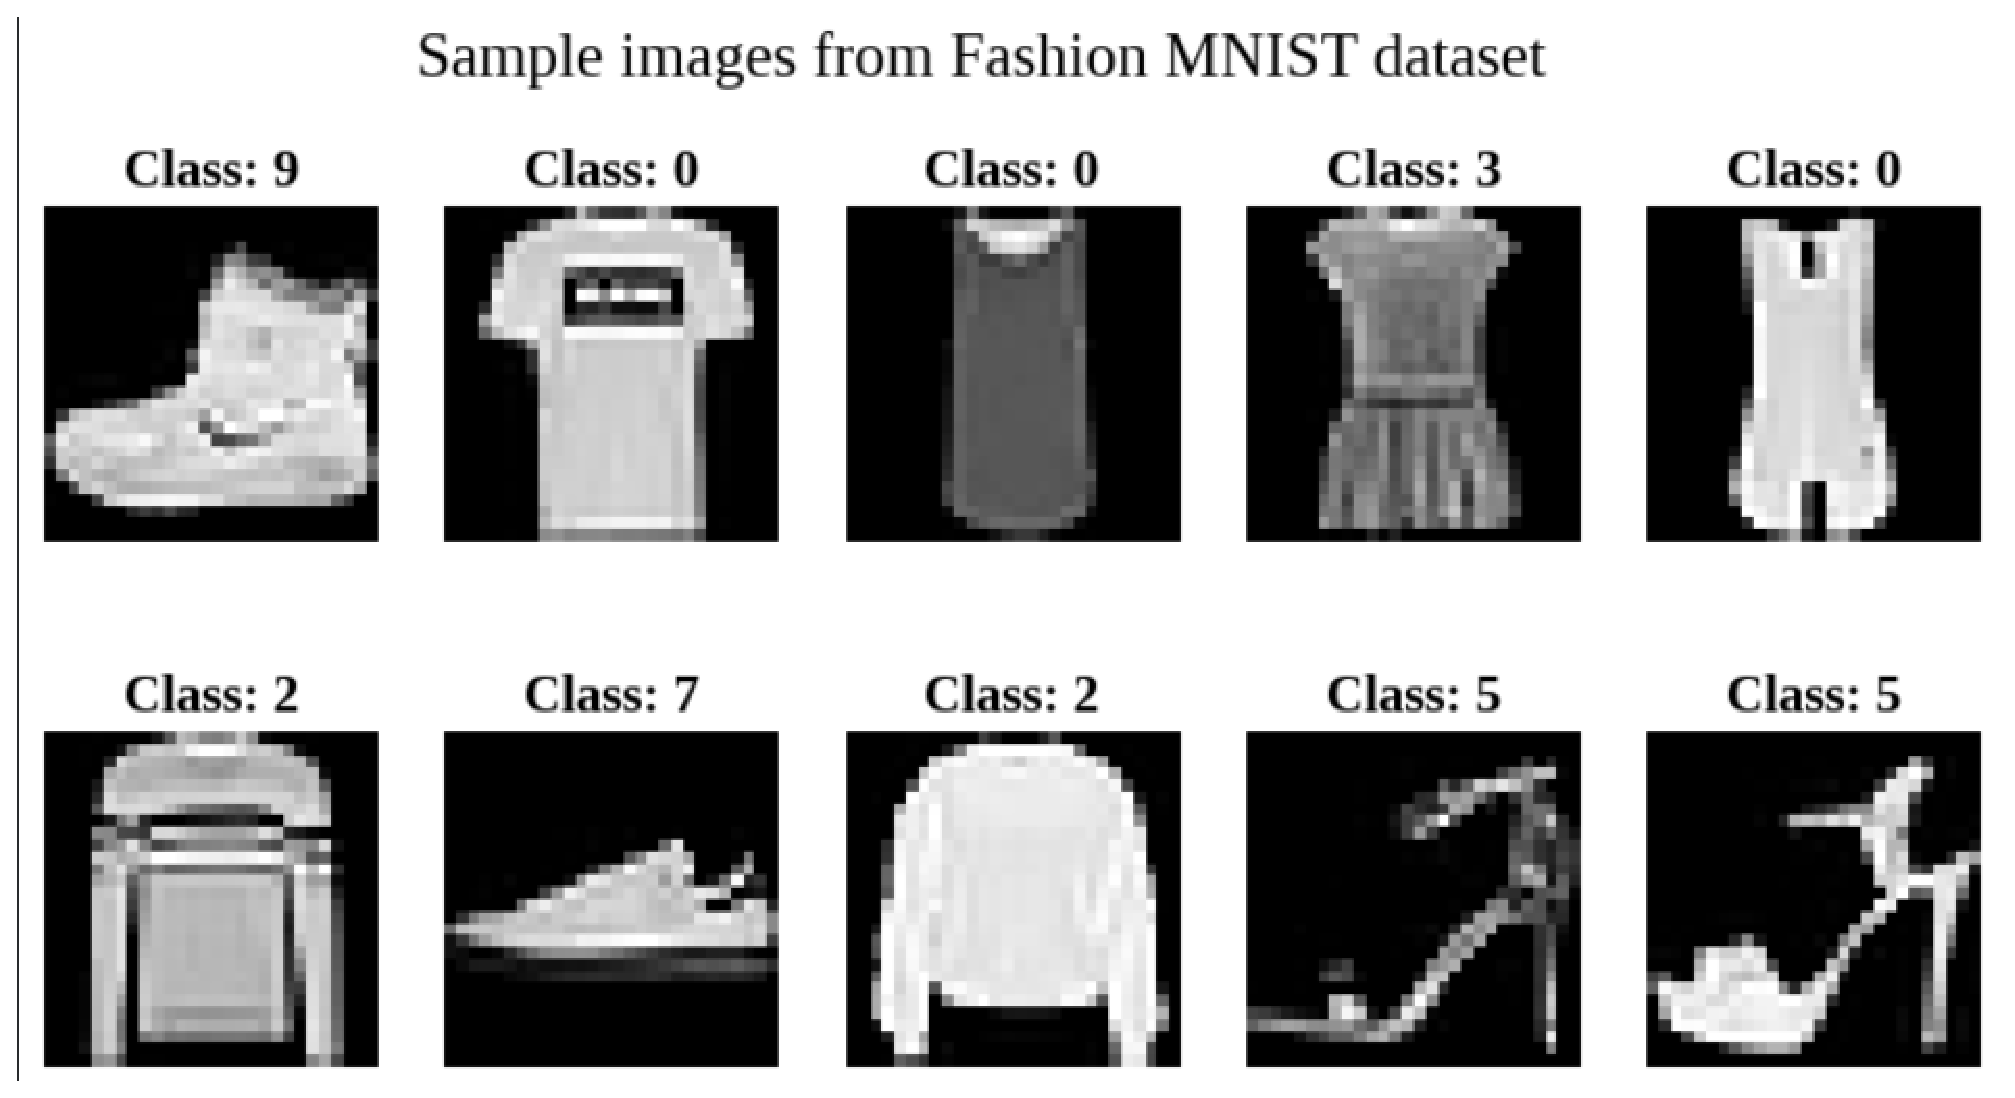
\includegraphics[width=0.5\textwidth]{SampleImages.eps}
    \caption{Sample Images}
    \label{fig:SampleImages}
\end{figure}

\noindent\textbf{Sample Images Inference:}\\
The sample images represent different fashion items with distinct shapes and patterns.
These variations help the model learn and distinguish between different clothing classes.
\begin{figure}[H]
    \centering
    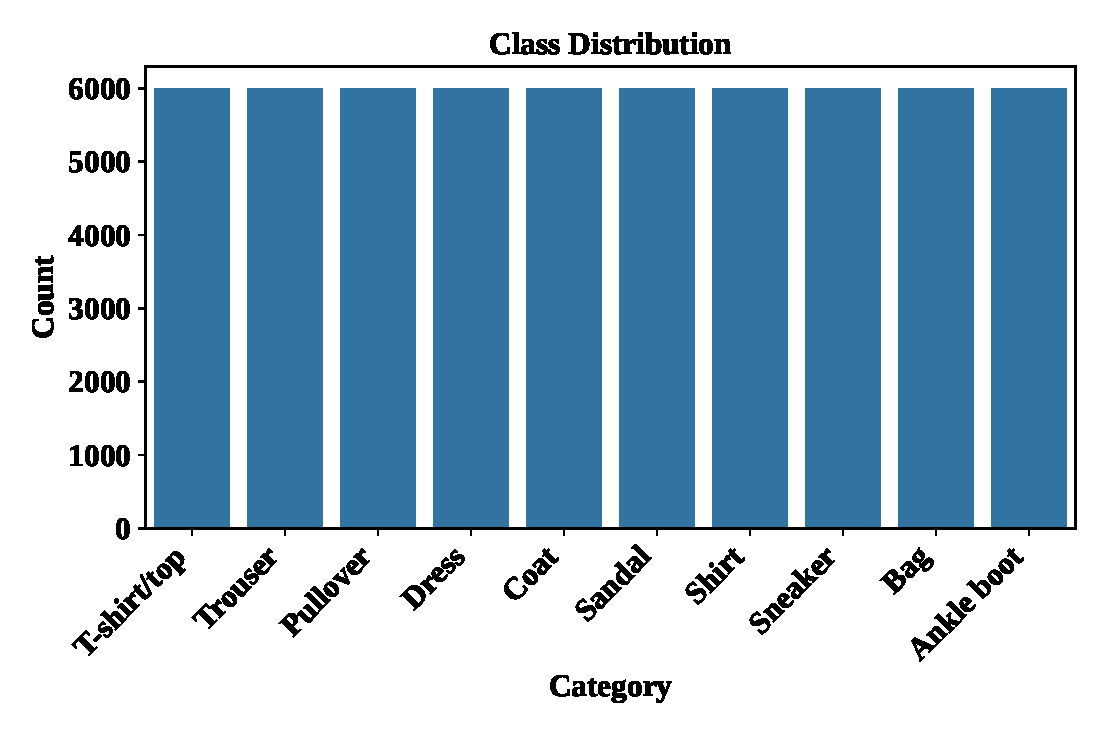
\includegraphics[width=0.5\textwidth]{ClassDistribution.eps}
    \caption{Class Distribution}
    \label{fig:ClassDistribution}
\end{figure}

\noindent\textbf{Class Distribution Inference:}\\
The plot shows that there exists 10 different fashion item classes.
Each class has 6000 samples.
\begin{figure}[H]
    \centering
    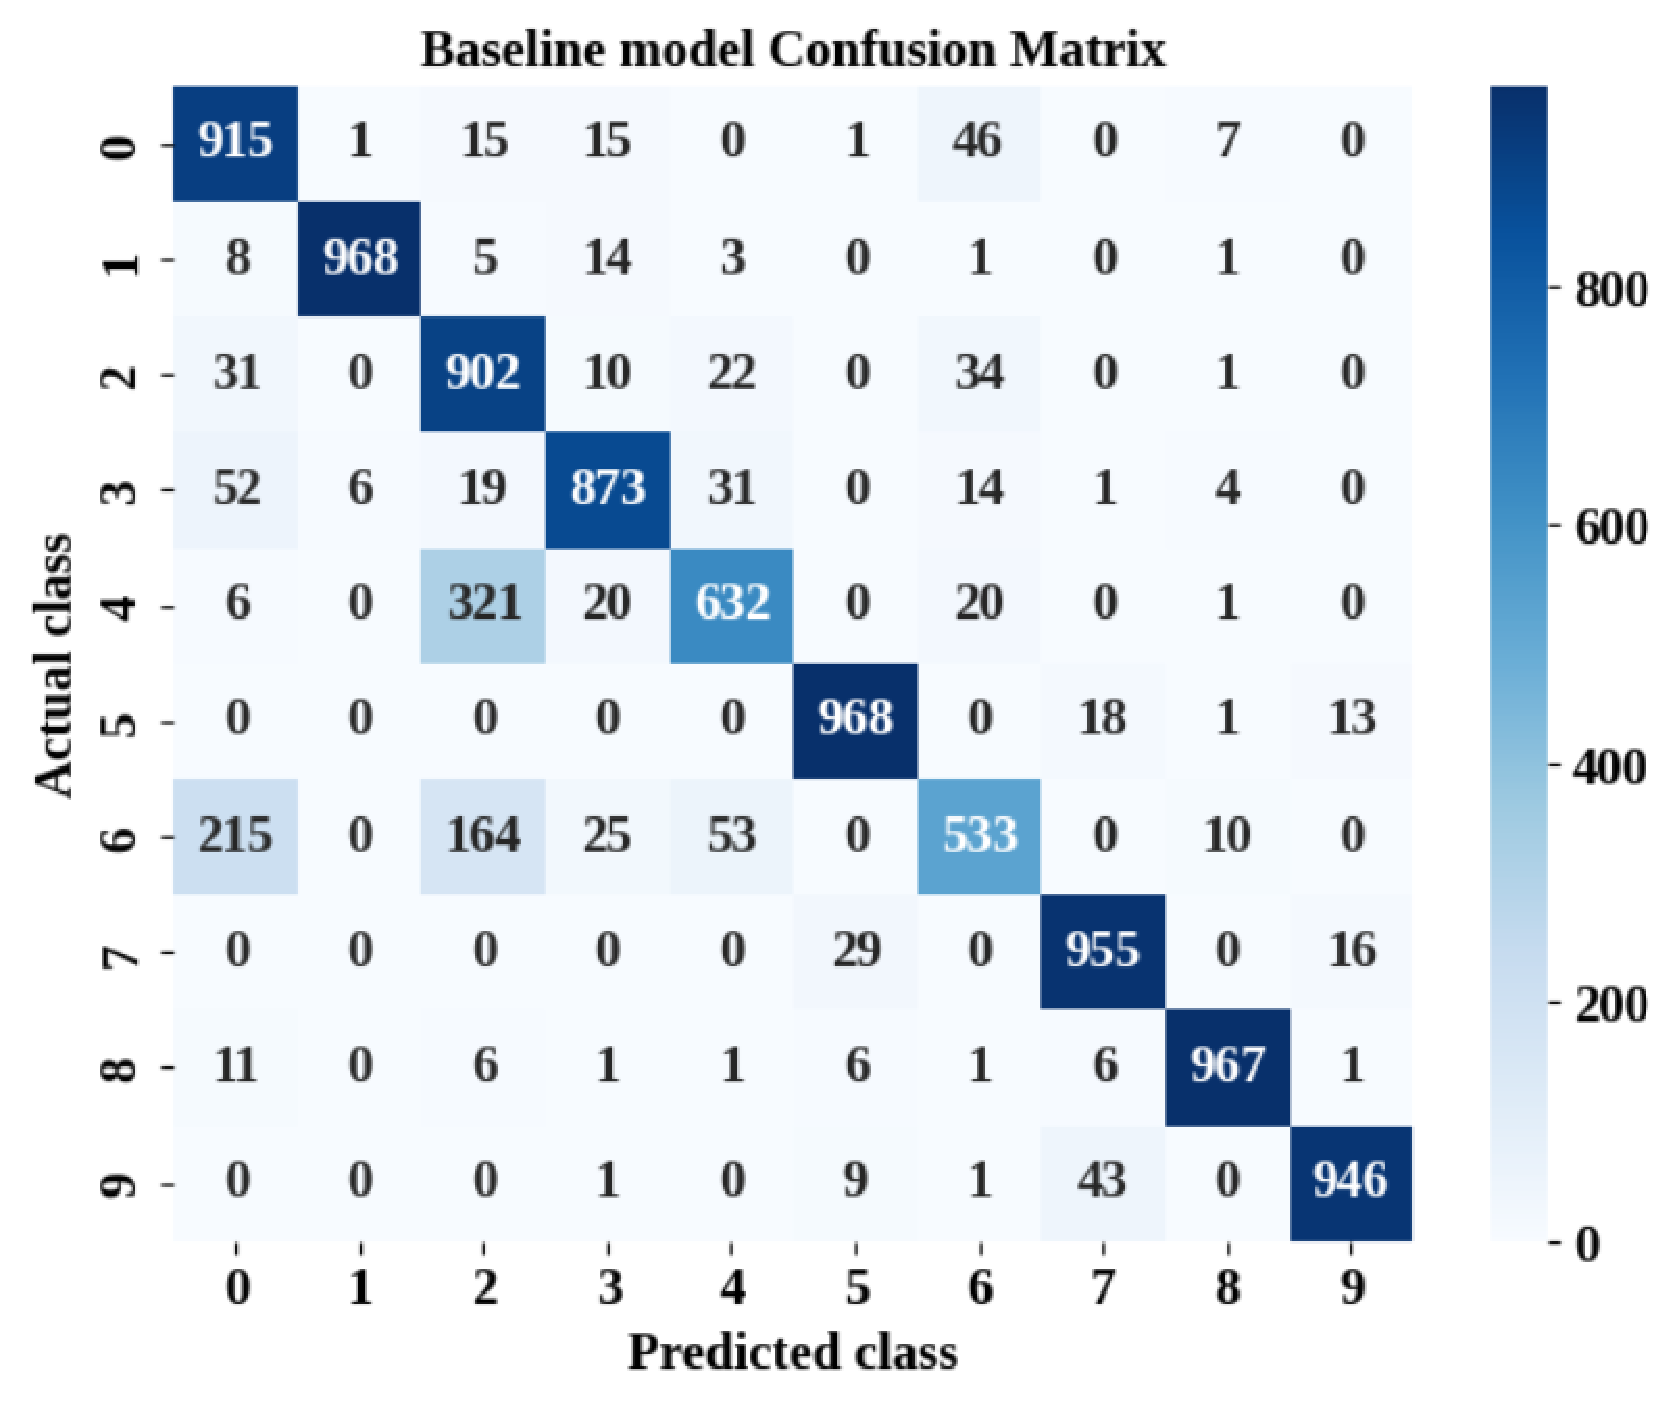
\includegraphics[width=0.5\textwidth]{BaselineModelConfusionMatrix.eps}
    \caption{Baseline Model ConfusionMatrix}
    \label{fig:BaselineModelConfusionMatrix}
\end{figure}

\noindent\textbf{Baseline Model Confusion Matrix Inference:}\\
The model correctly predicts most classes, performing best on classes 1, 5, 7, 8, and 9.
It misclassifies class 4 as class 2 and class 6 as class 2 or class 0 often.
\begin{figure}[H]
    \centering
    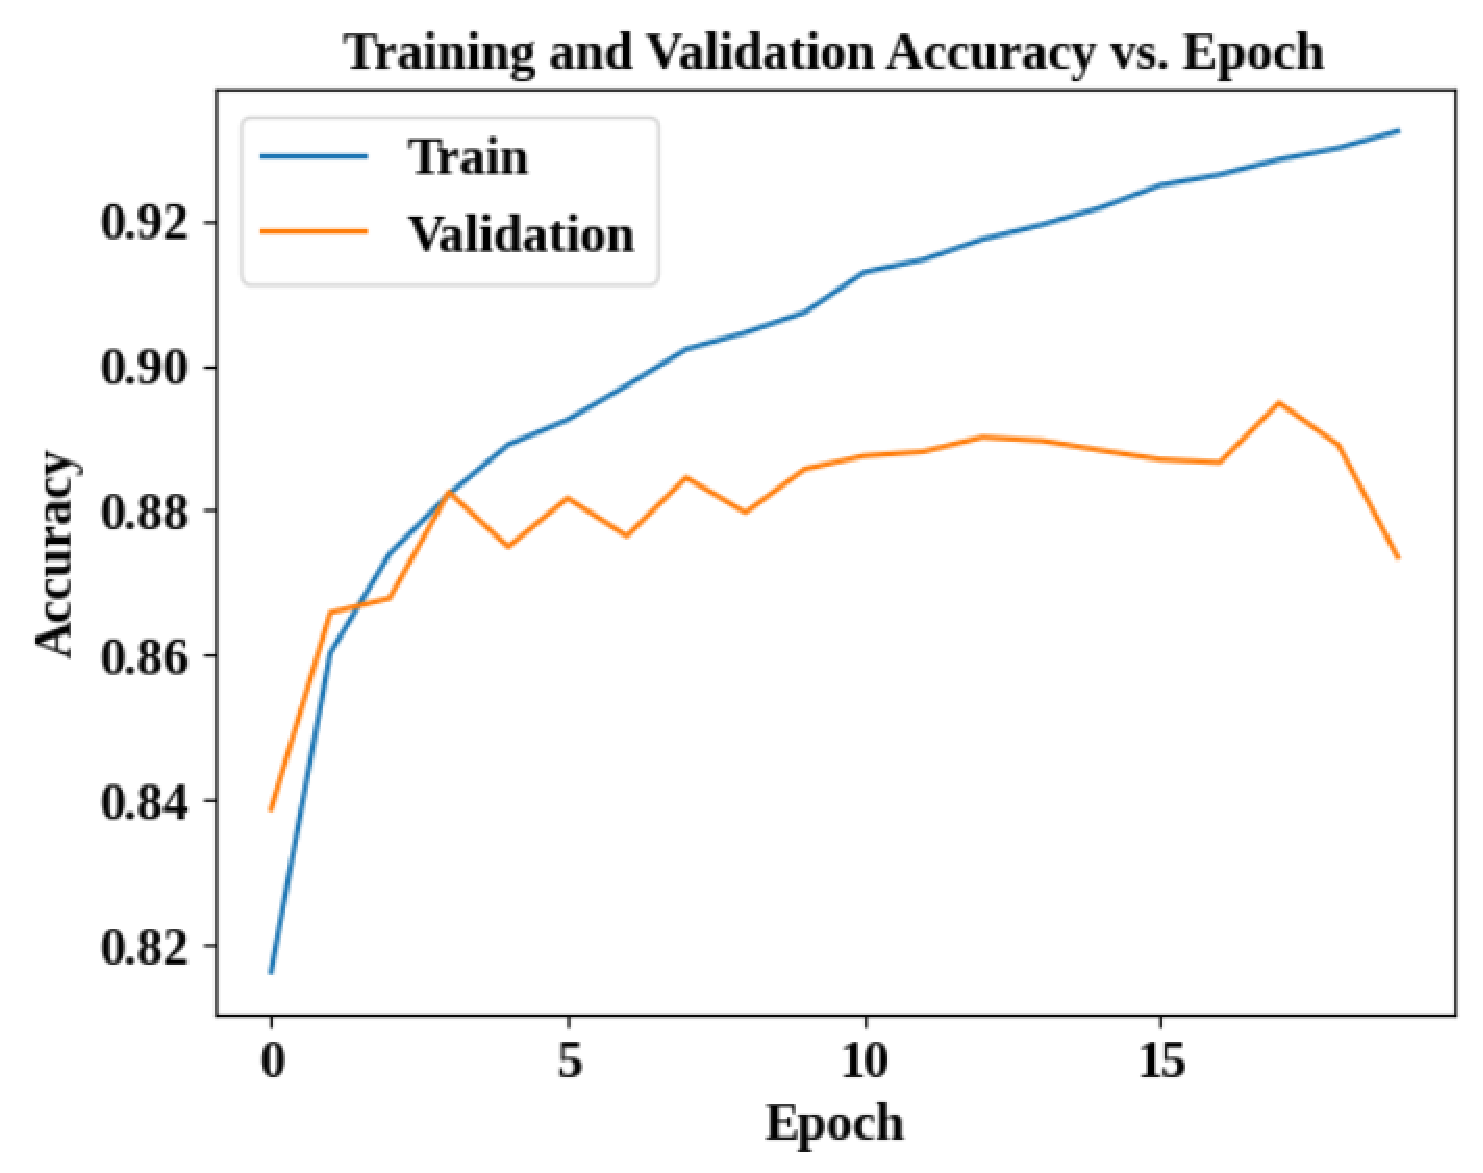
\includegraphics[width=0.5\textwidth]{TrainingValidationAccuracyVsEpoch.eps}
    \caption{Training, Validation Accuracy Vs Epoch}
    \label{fig:TrainingValidationAccuracyVsEpoch}
\end{figure}

\noindent\textbf{Training, Validation Accuracy Vs Epoch Inference:}\\
Training accuracy teadily increases throughout training, reaching over 93 percent showing the model is learning the training data well.
Validation accuracy plateaus around 89 percent after epoch 5 and drops sharply at the end indicating the model stops improving on unseen data and begins to overfit.
\begin{figure}[H]
    \centering
    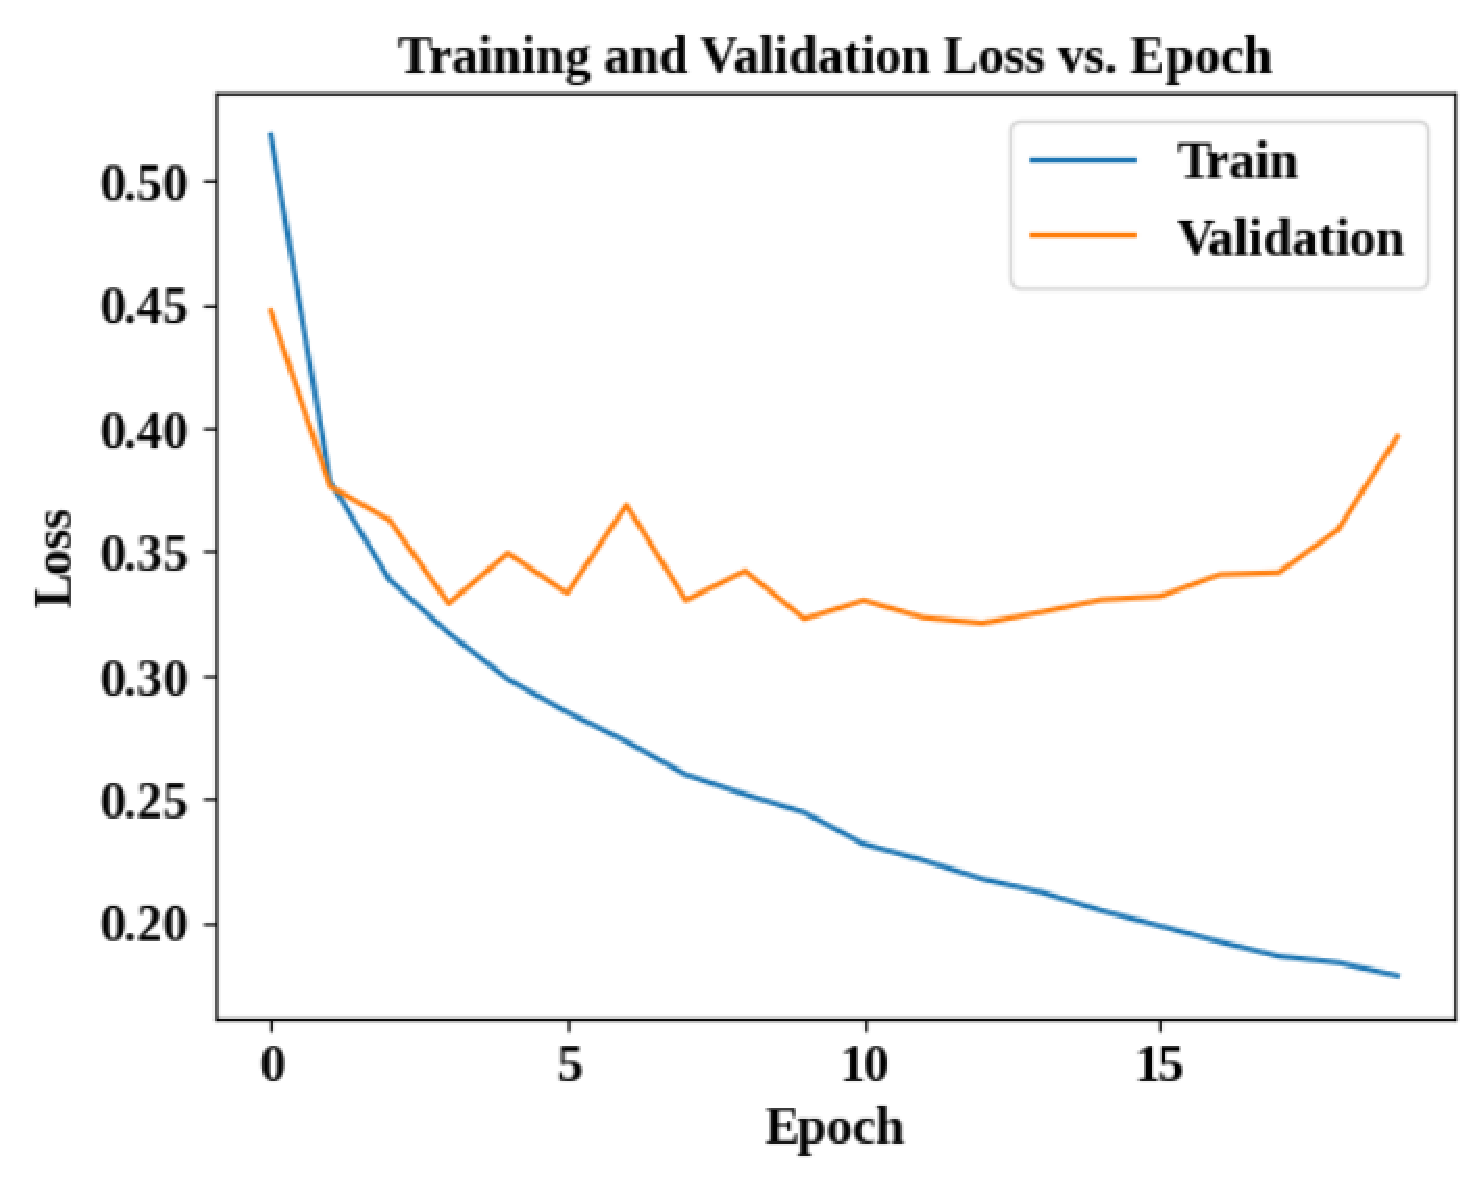
\includegraphics[width=0.5\textwidth]{TrainingValidationLossVsEpoch.eps}
    \caption{Training, Validation Loss Vs Epoch}
    \label{fig:TrainingValidationLossVsEpoch}
\end{figure}

\noindent\textbf{Training, Validation Loss Vs Epoch Inference:}\\
Training loss continuously decreases towards 0.18 showing consistent optimization on the training set.
Validation loss decreases initially but hits a minimum around epoch 10 and 15 and begins rising sharply, clearly confirming overfitting in later epochs.
\begin{figure}[H]
    \centering
    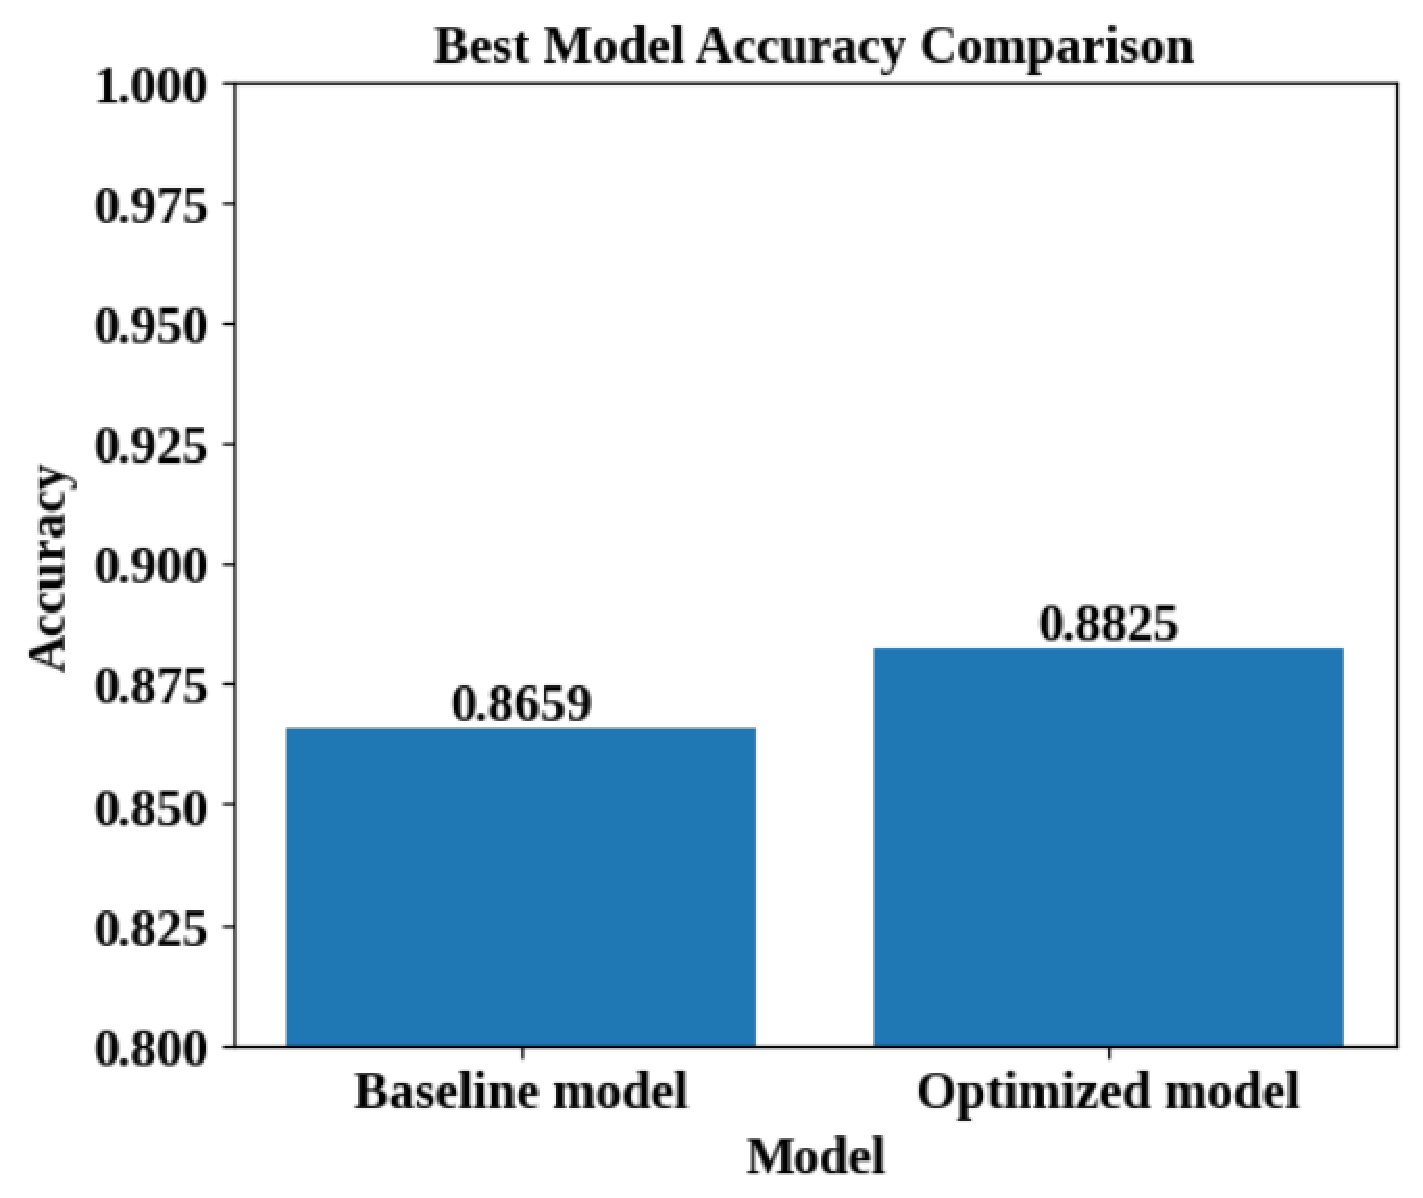
\includegraphics[width=0.5\textwidth]{BestModelAccuracyComparison.eps}
    \caption{Best Model Accuracy Comparison}
    \label{fig:BestModelAccuracyComparison}
\end{figure}
\noindent\textbf{Best Model Accuracy Comparison Inference:}\\
The optimized model achieved a higher accuracy of 88.25 percent compared to the baseline model's 86.59 percent.
This indicates that hyperparameter tuning improved the model's classification performance.

\section*{10. Additional Task}
Code the perceptron learning algorithm for the XOR gate using Python. Show the weights after each update. Plot the decision boundary after each weight update using Python's built-in packages. Analyze and identify the pattern that prevents the algorithm from converging.

\section{Source Code}
\url{https://github.com/ssvibitha/DeepLearningLab_2026-27/blob/main/Lab2_MLP/AdditionalTask_2.ipynb}

\section{Plots and Inference}
\begin{figure}[H]
    \centering
    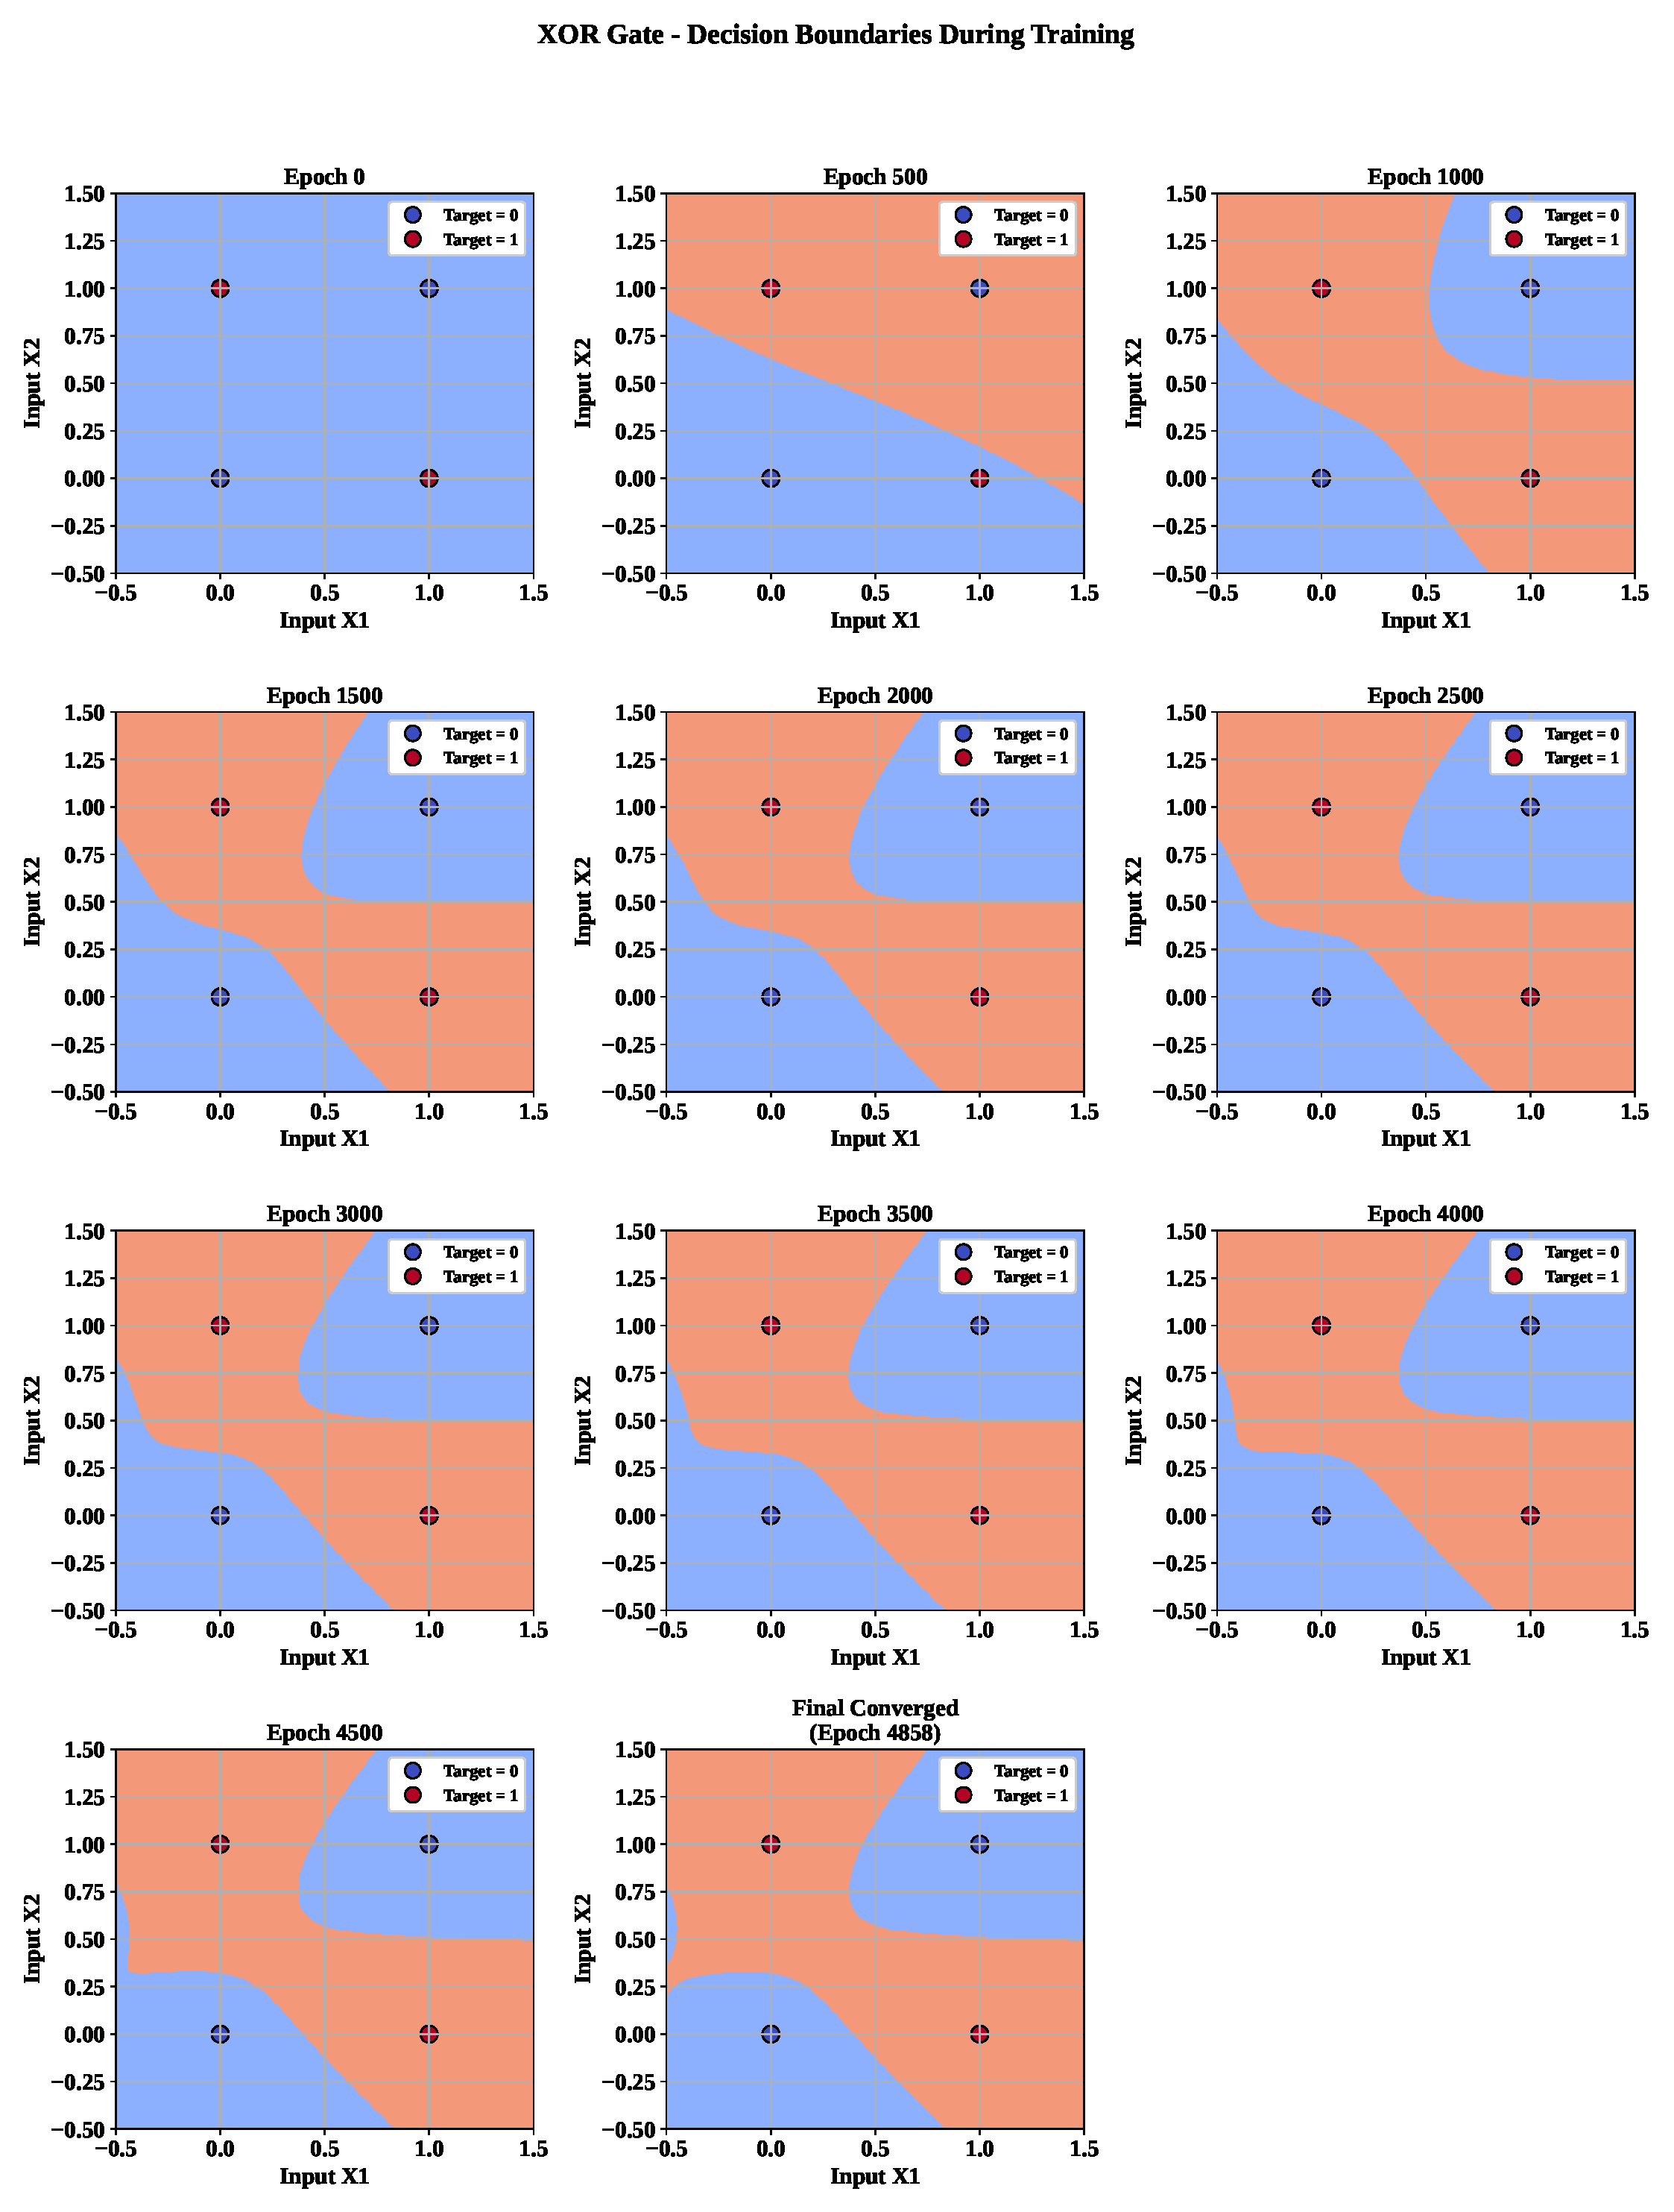
\includegraphics[width=0.9\textwidth]{MLP_XOR.eps}
    \caption{Multi-Layer Perceptron Training for XOR Gate}
    \label{fig:MLPTrainingXOR}
\end{figure}
\noindent\textbf{Multi-Layer Perceptron Training for XOR Gate Inference:}
\vspace{0.3cm}
\begin{itemize}

    \item The figure shows how the decision boundary changes during the training of a 
    Multi-Layer Perceptron for XOR gate. As training progresses, the model learns from 
    errors and adjusts its weights to create a better separation between the classes.
    \vspace{0.3cm}
    \item \textbf{Epoch 0: Initial State}
    \begin{itemize}
        \item At the beginning of training, the model starts with randomly initialized 
        weights.
        \item Since the model has not learned any patterns yet, it predicts the same 
        class for the entire input space, resulting in a single decision region.
    \end{itemize}
    \vspace{0.3cm}
    \item \textbf{Epoch 500: Initial Boundary Formation}
    \begin{itemize}
        \item A basic linear decision boundary starts to appear as the model begins 
        learning from the data.
        \item However, the boundary is not sufficient to classify the points correctly 
        because the given pattern requires a non-linear separation.
    \end{itemize}
    \vspace{0.3cm}
    \item \textbf{Epochs 1000--2500: Learning Non-Linear Patterns}
    \begin{itemize}
        \item As training continues, the hidden layers update their weights through 
        backpropagation.
        \item The decision boundary starts changing from a straight line into a curved 
        shape, allowing the model to learn more complex relationships.
        \item The model begins creating separate regions for correctly classifying the 
        points:
        \begin{itemize}
            \item \textbf{Target = 1:} $(0,1)$ and $(1,0)$
            \item \textbf{Target = 0:} $(0,0)$ and $(1,1)$
        \end{itemize}
    \end{itemize}
    \vspace{0.3cm}
    \item \textbf{Epochs 3000--4500: Refinement of Decision Regions}
    \begin{itemize}
        \item The model continues adjusting its weights to improve classification 
        accuracy.
        \item The decision boundaries become more defined and gradually move to better 
        separate the two classes.
        \item The network becomes more confident in classifying each input point 
        correctly.
    \end{itemize}
    \vspace{0.3cm}
    \item \textbf{Epoch 4858: Final Converged State}
    \begin{itemize}
        \item After several training iterations, the model reaches a stable state where 
        the decision boundaries correctly classify all the input points.
        \item The points $(0,1)$ and $(1,0)$ are classified as \textbf{Target = 1}, 
        while $(0,0)$ and $(1,1)$ are classified as \textbf{Target = 0}.
    \end{itemize}
    \vspace{0.3cm}
    \item \textbf{Training Significance}
    \begin{itemize}
        \item The movement of the decision boundary across epochs shows how the neural 
        network learns and improves through repeated weight updates.
        \item The formation of curved boundaries highlights the ability of hidden layers 
        to learn non-linear patterns, unlike a Single Layer Perceptron which can only 
        create linear boundaries.
        \item The final stable decision regions show that the network has successfully 
        learned the classification pattern and achieved convergence.
    \end{itemize}

\end{itemize}
\section*{11. Discussion}

Answer the following:

\begin{enumerate}
\item \textbf{Which optimization method was used?}\\
Randomized Search with Cross-Validation is used to find the best hyperparameters.
\item \textbf{Which hyperparameters were selected?}\\
The selected hyperparameters are
\begin{itemize}
        \item Hidden Layers: 3
        \item Hidden Neurons: 128
        \item Learning Rate: 0.001
        \item Batch Size: 32
        \item Optimizer: RMSprop
        \item Activation Function: tanh
        \item Epochs: 30
        \item Dropout: 0.2
    \end{itemize}
\item \textbf{Did optimization improve performance?}\\
Yes, after optimization the testing accuracy improved from 86.59 percent to 88.25 percent, along with improved precision, recall, and F1-score.
\item \textbf{Which hyperparameter had the greatest impact?}\\
The optimizer RMSprop and learning rate of 0.001 had the greatest impact helping improve the model's performance.
\item \textbf{Compare Grid Search and Randomized Search.}\\
Grid Search tests every possible combination of hyperparameters. Hence it is more computationally expensive.
Randomized Search tests a random subset of combinations, and finds good results with less computation.
\item \textbf{Recommend the best MLP configuration.}\\
MLP configuration with 3 hidden layers, 128 neurons, tanh activation, RMSprop optimizer, learning rate 0.001, batch size 32, dropout 0.2, and 30 epochs is recommended as it achieved the highest testing accuracy of 88.25 percent.
\end{enumerate}


\section*{12. Conclusion}
The experiment successfully trained and evaluated an MLP classifier on the Fashion MNIST dataset and trained MLP on XOR gate.
Hyperparameter tuning in training the Fashion MNIST dataset improved the model's accuracy and overall classification performance, resulting in a more effective classifier.


\section*{13. References}
\begin{enumerate}
\item Goodfellow et al., \emph{Deep Learning}.
\item Bishop, \emph{Pattern Recognition and Machine Learning}.
\item Haykin, \emph{Neural Networks and Learning Machines}.
\item Fashion-MNIST Dataset.
\item TensorFlow/Keras Documentation.
\end{enumerate}

\end{document}
